\IfFileExists{figures/kuzlog.pdf}{
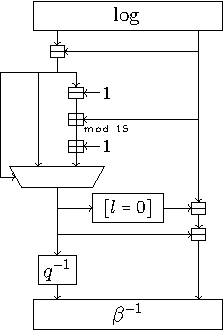
\includegraphics[height=\HEIGHT]{figures/kuzlog.pdf}
}{
    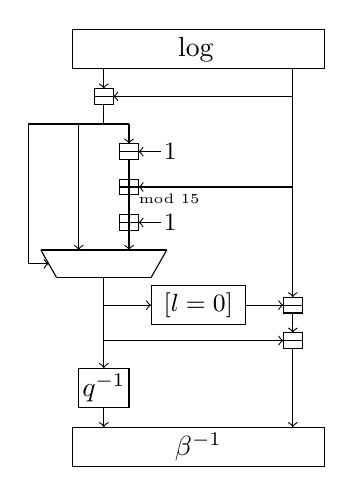
\begin{tikzpicture}[xscale=0.8,yscale=-0.5]
                % \draw (0.0,0.0) node[anchor=south] {$l$};
                % \draw (3.0,0.0) node[anchor=south] {$r$};
                % \draw[->] (0.0,0.0) -- (0.0,0.5);
                % \draw[->] (3.0,0.0) -- (3.0,0.5);
                \draw (-0.5,0.5) rectangle (3.5,1.5) node[pos=0.5] {$\log{}$};
                \draw[->] (0.0,1.5) -- (0.0,2.0);
                \draw (-0.15,2.0) rectangle (0.15,2.4);
                \draw (-0.15,2.2) -- (0.15,2.2);
                \draw (3.0,1.5) -- (3.0,2.2);
                \draw[->] (3.0,2.2) -- (0.15,2.2);
                \draw (0.0,2.4) -- (0.0,2.9);
                \draw (3.0,2.2) -- (3.0,2.9);
                \draw (0.0,2.9) -- (-0.4,2.9);
                \draw (0.0,2.9) -- (0.4,2.9);
                \draw (-0.4,2.9) -- (-1.2,2.9);
                \draw[->] (0.4,2.9) -- (0.4,3.4);
                \draw (0.25,3.4) rectangle (0.55,3.8);
                \draw (0.25,3.6) -- (0.55,3.6);
                \draw (0.8,3.6) node[anchor=west] {\small 1};
                \draw[->] (0.9,3.6) -- (0.55,3.6);
                \draw (0.4,3.8) -- (0.4,4.3);
                \draw (0.25,4.3) rectangle (0.55,4.7);
                \draw (0.4,4.3) -- (0.4,4.7);
                \draw (0.25,4.5) -- (0.55,4.5);
                \draw (3.0,2.9) -- (3.0,4.5);
                \draw[->] (3.0,4.5) -- (0.55,4.5);
                \draw (0.4,4.8) node[anchor=west] {\tiny mod 15};
                \draw (0.4,4.7) -- (0.4,5.2);
                \draw (0.25,5.2) rectangle (0.55,5.6);
                \draw (0.4,5.2) -- (0.4,5.6);
                \draw (0.25,5.4) -- (0.55,5.4);
                \draw (0.8,5.4) node[anchor=west] {\small 1};
                \draw[->] (0.9,5.4) -- (0.55,5.4);
                \draw (-0.4,2.9) -- (-0.4,5.6);
                \draw[->] (-0.4,5.6) -- (-0.4,6.1);
                \draw[->] (0.4,5.6) -- (0.4,6.1);
                \draw (-1.0,6.1) -- (1.0,6.1);
                \draw (1.0,6.1) -- (0.75,6.8);
                \draw (0.75,6.8) -- (-0.75,6.8);
                \draw (-0.75,6.8) -- (-1.0,6.1);
                %\path (-0.75,6.1) -- (0.75,6.8) node[pos=0.5] {\small $[l = 0]$};
                \path (-0.75,6.1) -- (0.75,6.8) node[pos=0.5] {};
                \draw (-1.2,2.9) -- (-1.2,6.45);
                \draw[->] (-1.2,6.45) -- (-0.875,6.45);
                \draw (3.0,4.5) -- (3.0,6.8);
                \draw (0.0,6.8) -- (0.0,7.5);
                \draw[->] (3.0,6.8) -- (3.0,7.3);
                \draw (2.85,7.3) rectangle (3.15,7.7);
                \draw (2.85,7.5) -- (3.15,7.5);
                \draw[->] (0.0,7.5) -- (0.75,7.5);
                \draw (0.75,7.0) rectangle (2.25,8.0) node[pos=0.5] {\small $[ l = 0 ]$};
                \draw[->] (2.25,7.5) -- (2.85,7.5);
                \draw (0.0,7.5) -- (0.0,8.4);
                \draw[->] (3.0,7.7) -- (3.0,8.2);
                \draw (2.85,8.2) rectangle (3.15,8.6);
                \draw (2.85,8.4) -- (3.15,8.4);
                \draw[->] (0.0,8.4) -- (2.85,8.4);
                \draw[->] (0.0,8.4) -- (0.0,9.1);
                \draw (-0.4,9.1) rectangle (0.4,10.1) node[pos=0.5] {$q^{-1}$};
                \draw[->] (0.0,10.1) -- (0.0,10.6);
                \draw[->] (3.0,8.6) -- (3.0,10.6);
                \draw (-0.5,10.6) rectangle (3.5,11.6) node[pos=0.5] {$\beta^{-1}$};
                % \draw[->] (0.0,11.6) -- (0.0,12.1);
                % \draw[->] (3.0,11.6) -- (3.0,12.1);
            \end{tikzpicture}
}
